% =============================================================================
% File:  opening.tex -- 
% Author(s): Sebastien Varrette (sebastien.varrette@uni.lu)
% Time-stamp: <Tue 2015-06-16 09:22 svarrette>
% 
% Copyright (c) 2015 Sebastien Varrette<Sebastien.Varrette@uni.lu>
% 
% For more information:
% - LaTeX: http://www.latex-project.org/
% - Beamer: https://bitbucket.org/rivanvx/beamer/
% - LaTeX symbol list:
% http://www.ctan.org/tex-archive/info/symbols/comprehensive/symbols-a4.pdf
% =============================================================================

\documentclass{beamer}
% \documentclass[draft]{beamer}
\usepackage{_style}
\usepackage{wrapfig}
\usepackage{setspace}
% The key part to use my theme -- if you precise nothing, the image that
% illustrate the slides is assumed to be images/slides_image.jpg
\usetheme[image=logos/logo_hpc-shool2015.pdf]{Falkor}

% Not integrated in my theme as not everybody wants that
\AtBeginSection[]
{
  \frame{
    \frametitle{Summary}
    {\scriptsize\tableofcontents[currentsection]}
  }
}

\graphicspath{{images/}} % Add this directory to the searched paths for graphics


%%%%%%%%%% Header %%%%%%%%%%%%
\title{UL HPC School June 2015}
\subtitle{Opening Session}

\author{Sebastien Varrette}
\institute[PCOG Research unit]{
  Parallel Computing and Optimization Group (\href{http://pcog.uni.lu}{PCOG}),
  University of Luxembourg (\href{http://www.uni.lu}{UL}), Luxembourg
}

% Mandatory to **declare** a logo to be placed on the bottom right -- normally the
% university logo. ADAPT ACCORDINGLY:
\pgfdeclareimage[height=0.8cm]{logo}{logos/logo_UL.pdf}

\date{}

%%%%%%%%%%%%% Body %%%%%%%%%%%%%%%
\begin{document}

\begin{frame}
  \vspace{2.5em}
  \titlepage
\end{frame}

% ......
% \frame{
%   \frametitle{Summary}
%   {\scriptsize
%     \tableofcontents
%   }
% }

% ======================== 
% \input{_content.md} % Markdown content
% ======================== 

\frame{
  \frametitle{Welcome to the UL HPC School}

  \begin{itemize}
    \item \emph{Third edition} after successful 2014 and March 2015 editions
      \begin{itemize}
          \itemhook main event of 2015 with basic + advanced tutorials
          \itemhook following the newcomer edition of March
          \itemhook 46 registered participants
          \itemhook 7 distinct speakers
          \begin{itemize}
            \item supported by some of the leading UL computational scientists
          \end{itemize}
          \itemhook Open and public access -- content on
          \href{https://github.com/ULHPC/tutorials}{GitHub}
      \end{itemize}
      \hfill
\includegraphics[height=3em]{blog-github.png}
  \end{itemize}
}

\frame{
  \frametitle{UL HPC School Overview}

  \begin{itemize}
    \item \textbf{6 keynotes} (including user's session)
    \item \textbf{15 practical sessions across 3 tracks}
      \begin{itemize}
          \itemhook focusing on observed daily usage of the platform
          \itemhook basics, sequential \& parallel jobs, specific applications targeted
          (Matlab, R, bioinfo, engineering, physics, chemistry)
      \end{itemize}
  \end{itemize}
}

\frame{
  \frametitle{Agenda - Day 1 (June 25th)}

  \centering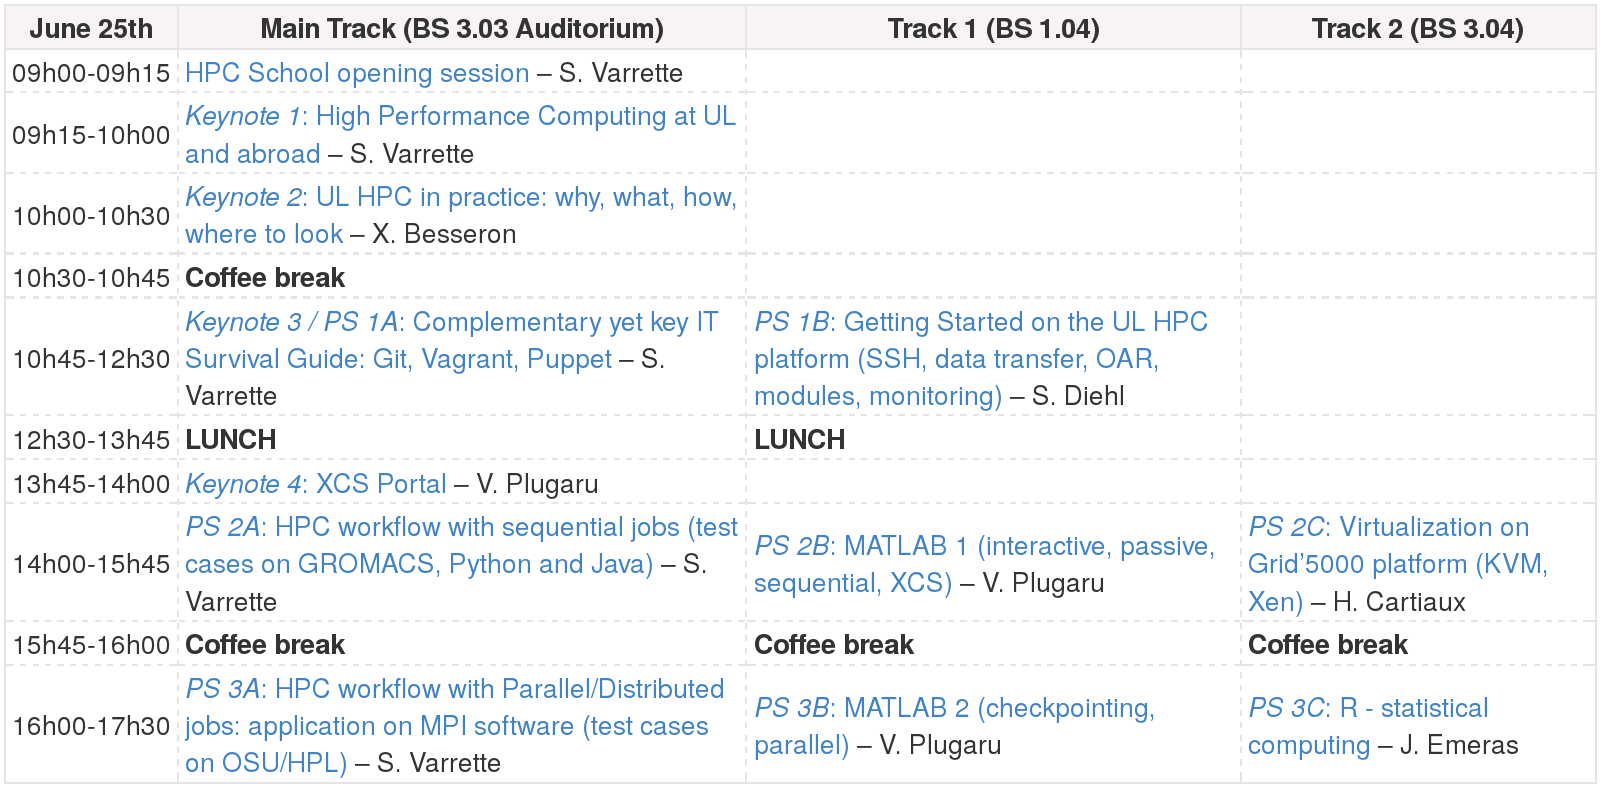
\includegraphics[width=0.95\textwidth]{agenda_day1}

}

\frame{
  \frametitle{Agenda - Day 2 (June 26th)}

  \centering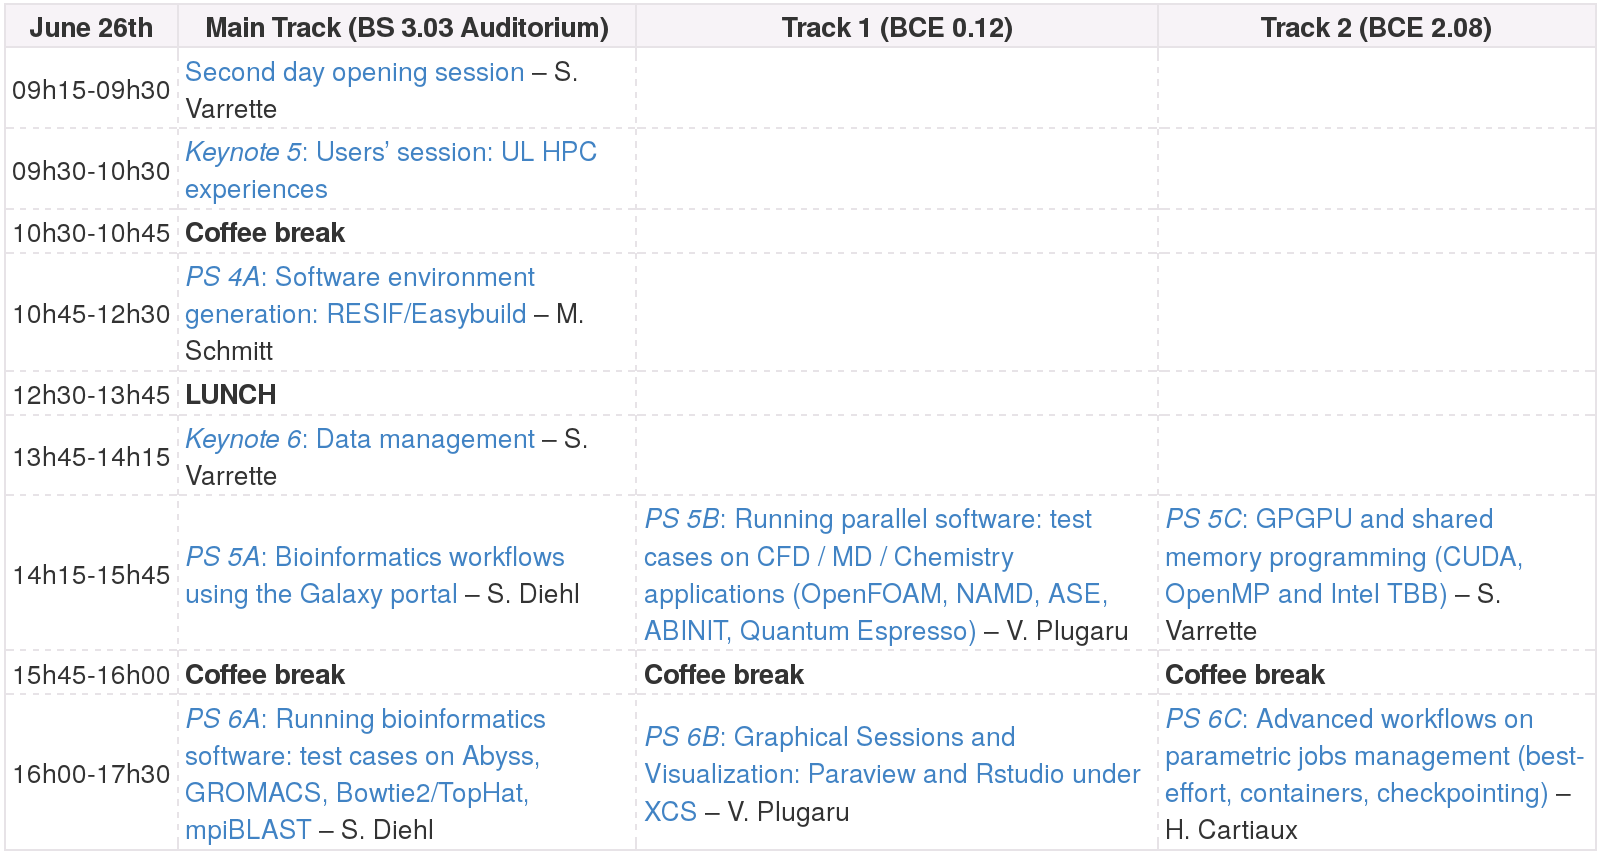
\includegraphics[width=0.95\textwidth]{agenda_day2}
}

\frame{
  \begin{center}

      {\Large \url{http://hpc.uni.lu/hpc-school}}
      \vfill
      \begin{description}
        \item[Github Tutorials:] \hfill
          \myurl{https://github.com/ULHPC/tutorials}
        \item[UL HPC website] \hfill
          \myurl{https://hpc.uni.lu}
      \end{description}
  \end{center}
}

\frame{
  \frametitle{The UL HPC Team}
  \begin{spacing}{0.5}
  
   \begin{columns}[T] 
    \begin{column}[T]{0.2\textwidth}
       \hfill\includegraphics[width=0.6\textwidth]{{pascal.bouvry}.jpg} \\
       \hfill\includegraphics[width=0.6\textwidth]{{sebastien.varrette}.jpg} \\
       \hfill\includegraphics[width=0.9\textwidth]{{hyacinthe.cartiaux}.jpg}\\
       \hfill\includegraphics[width=0.9\textwidth]{{valentin.plugaru}.jpg}\\
       \hfill\includegraphics[width=0.9\textwidth]{{sarah.diehl}.jpg}\\
    \end{column}
    \begin{column}[T]{0.8\textwidth}
     {\tiny \textbf{Pascal Bouvry} is a full professor of the \href{http://fstc.uni.lu}{FSTC}
     and the head of the \href{http://wwwen.uni.lu/recherche/fstc/interdisciplinary_lab_for_intelligent_and_adaptive_systems_ilias/}{ILIAS} 
     research unit and the \href{http://wwwen.uni.lu/formations/fstc/doctoral_school_of_computer_science_and_computer_engineering}{DS-CSCE} 
     doctoral school. His team (\href{http://pcog.uni.lu}{PCOG}) is composed of 25 researchers working on Parallel computing and Optimization 
     applied to Cloud Computing and HPC (scheduling, energy-efficiency, security), Ad-Hoc Networks (Vanets simulation and service optimization)
     and Biology (gene sequencing, regulatory networks, protein folding).} \\
    
     \vspace{2ex}
     {\tiny \textbf{S\'ebastien Varrette}, PhD, is a Research Associate in Prof. Bouvry's team since 2007. Along with Prof. Bouvry, he
     defined and set up the global HPC initiative of the UL in 2007. In this context, he is managing the sysadmin team that maintain 
     and extend the platform. In parallel, his research work focuses on Distributed Computing Platforms (clusters, grids or clouds),
     with a particular interest on the security and performance evaluation of distributed or parallel executions.}\\
    
     \vspace{1ex}
     {\tiny \textbf{Hyacinthe Cartiaux} joined the HPC team in 2011 to set up the Grid'5000 Luxembourg site and has since been involved with all 
     the HPC infrastructure of the UL, and other external services such as the Gforge. His interests cover IT automation and devops techniques, 
     HPC \& Grid Computing.}\\
     
     \vspace{2ex}
     {\tiny \textbf{Valentin Plugaru} is an HPC engineer part of the HPC team since 2014. Beginning with 2012 he has collaborated with Prof. 
     Bouvry's team on research in Energy Efficiency and Performance Evaluation of HPC/Cloud environments. His general interests span R\&D 
     in High Performance Computing, Grid and Cloud Computing.} \\
     
     \vspace{2.5ex}
     {\tiny \textbf{Sarah Diehl} is a bioinformatician and joined the LCSB BioCore in 2015 as an HPC systems administrator. Her goal is to 
     bridge the gap between researchers and IT specialists. She is experienced in data management, next-generation sequencing analysis and 
     development of analysis pipelines.}\\
   \end{column}
  \end{columns}
  
 \end{spacing}
}


\frame[containsverbatim,t]{
  \frametitle{Top 2014 User reports}

  \begin{itemize}
    \item Total \textbf{used} resources in 2014: \emph{1417 years} %\hfill{\tiny since 2008}
    \item \emph{Up 33\%} compared with 2013
  \end{itemize}

   \begin{center}
      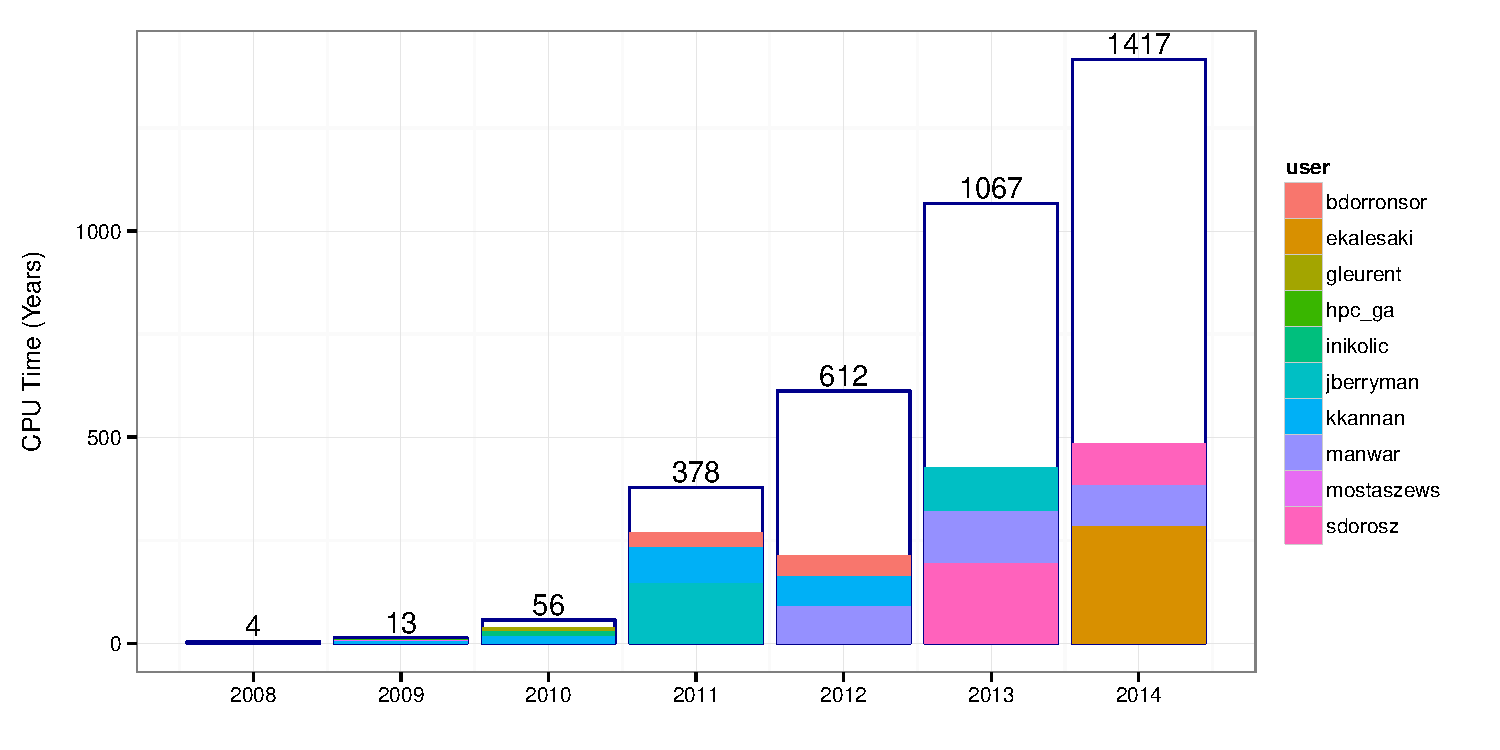
\includegraphics[width=0.9\textwidth]{platform_used_with_users_2014.pdf}
  \end{center}
}

\frame[containsverbatim,t]{
  \frametitle{Top 2014 User reports}
  {\tiny
\begin{verbatim}
            login          total_asked  total_used CPUHour used                    
        --  ---------      -----------  ---------- -----------------------------
        1   ekalesaki      51975866400  8970447983 0285 years 096 days 15:06:23
        2   manwar         7847452800   3179608677 0101 years 278 days 00:37:57
        3   sdorosz        6205410000   3162397174 0101 years 078 days 19:39:34
        4   amolinasanchez 24369418958  2207770186 0070 years 351 days 21:29:46
        5   jberryman      9067514400   1913896245 0061 years 237 days 13:50:45
        6   hmiranda       35220902400  1662562243 0053 years 250 days 14:50:43
        7   sokawa         7206109200   1086009034 0035 years 152 days 13:10:34
        8   pmay           3734942400   1064860651 0034 years 272 days 18:37:31
        9   akalantari     7572693600   1058740031 0034 years 201 days 22:27:11
        10  snielsen       5725191600   1030758605 0033 years 243 days 01:50:05
        11  mdiarra        164418453000 1028947965 0033 years 222 days 02:52:45
        12  ahunegnaw      1557208800   976436531  0031 years 345 days 08:22:11
        13  jmuszynski     2814051551   951645828  0031 years 058 days 10:03:48
        14  dkim           125761759200 858230347  0028 years 073 days 05:19:07
        15  skillcoyne     13590576000  853731503  0028 years 021 days 03:38:23
\end{verbatim}
    }

    \begin{lstlisting}[basicstyle=\tiny,language=R,numbers=none]
## Function to convert cpuhour (in s) into a readable time formating
getTime <- function(x) {
  str = format(as.POSIXct('0001-01-01 00:00:00') + x, "%Y years %j days %H:%M:%S")
  return(str)
}
\end{lstlisting}

}


% ======================== END =========================
% \section*{Thank you for your attention...}
% \frame{
%   \frametitle{Questions?}
%   % ~~~~~~~~~~~~~~
%   \begin{columns}
%     \column{0.5\textwidth}
%     % \emph{Contact}\\
%     {\tiny
%       \emph{Sebastien Varrette}\\
%       ~~~~ \textit{mail:} \href{mailto:sebastien.varrette@uni.lu}{sebastien.varrette@uni.lu}\\
%       ~~~~ Office E-007\\
%       ~~~~ Campus Kirchberg\\
%       ~~~~ 6, rue Coudenhove-Kalergi\\
%       ~~~~ L-1359 Luxembourg
% 
%     }
%     \column{0.5\textwidth}
%     % \scalebox{8}{\emph{?}}
%     
\includegraphics[width=1.5in]{question.jpg}
%   \end{columns}
%   % Below is the table of content over 2 columns
%   \vfill
%   \begin{multicols}{2}
%     {\tiny \tableofcontents}
%   \end{multicols}
% 
% }

\newcounter{finalframe}
\setcounter{finalframe}{\value{framenumber}}

% %.......
% \frame{
%   \frametitle{}
%   \vfill
%   \centering \LARGE Appendix\footnote{notice the slide number below...}
%   \vfill
% }

\setcounter{framenumber}{\value{finalframe}}

\end{document}

% ~~~~~~~~~~~~~~~~~~~~~~~~~~~~~~~~~~~~~~~~~~~~~~~~~~~~~~~~~~~~~~~~
% eof
% 
% Local Variables:
% mode: latex
% mode: flyspell
% mode: visual-line
% TeX-master: "opening.tex"
% End:
